\documentclass[a4paper,12pt]{report}
\textheight=24cm
\textwidth=15cm

\usepackage{fancyhdr} 		%Headers and footers
\setlength{\headheight}{15pt}
\usepackage{setspace} 		%Line settings

%\usepackage{etoolbox}
%\makeatletter
%\patchcmd{\@makechapterhead}{50\p@}{0pt}{}{}
%\patchcmd{\@makeschapterhead}{50\p@}{0pt}{}{}
%\makeatother

\usepackage{titlesec} %Load this package to reduce the white space before and after chapter heading
\titleformat{\chapter}[display]
{\normalfont\huge\bfseries}{\chaptertitlename\ \thechapter}{20pt}{\Huge}
\titlespacing{\chapter}{0pt}{0pt}{20pt} % {command}{left}{before sep} {after sep}[right] default = {0pt}{50pt}{40pt}

\usepackage{color,graphicx} %Add colour to text and further arguments for graphics
\usepackage{caption}			%Subfigures over a page
\usepackage{subcaption}		%Subfigures over a page
\usepackage{url} 					%Allows you to add urls
%\usepackage{courier}			%Use courier font
\usepackage{kpfonts}
\usepackage{gensymb}			%Allows you to use \degree
\usepackage{tabulary}			%Allows you to wrap text in a table column
\usepackage{array}				%Needed for some functions in tabular
\usepackage{fixltx2e} 		%Allows you to use \textsubscript in tables
\usepackage{float}				%Places float at precisely the location in the LaTex code
\usepackage{nameref}			%Allows you to name chapter in reference rather than number
\usepackage[font=small, labelfont=bf]{caption} %Small captions in bold
\usepackage{booktabs}			%Allows you to use \toprule etc when converting excel tables to latex
\usepackage{longtable, lscape}		%Tables can span across multiple pages
\usepackage{tabu}
\newcommand{\ToDo}[1]{\textcolor{red}{\textsf{\textbf{#1}}}} %Creates a new command that hightlights text in red
%\usepackage[round]{natbib} 			%Allows you to work with author-year citations
\usepackage[titletoc,title]{appendix} %Allows partial titletoc in appendix, must be installed before hyperref package
\usepackage{titletoc} %Allows partial titletoc in appendix, must be installed before hyperref package
\usepackage[colorlinks=false]{hyperref} %Citations are turned into hypertext links
\usepackage{rotating} %Allows you to rotate floats
\usepackage{rotfloat} %Allows [H] to be used when rotating floats
\usepackage{setspace} %Set spacing in longtable
\usepackage{multirow} %Multirows in tables
\usepackage[backend=bibtex, style=authoryear, maxcitenames=2, mincitenames=1, minbibnames=10, maxbibnames=10, dashed=false]{biblatex} %References
\addbibresource{ThesisBibliography.bib} %Location of references
\renewbibmacro{in:}{} %Suppress the use of "`in"' before the journal title in bibliography
\DeclareNameAlias{sortname}{last-first} %Display all authors in biblopgraphy as last name followed by first
\renewcommand*{\bibpagespunct}{\addcolon\space} %colon instead of comma before pages in bibliography
\AtEveryBibitem{\clearfield{number}} %remove number field from bibliography


\pagestyle{fancy} 				%Change the style of the current page
\renewcommand{\chaptermark}[1]{\markboth{#1}{}} %Print the name of the chapter
\renewcommand{\sectionmark}[1]{\markright{\thesection\ #1}} %Print the name of the section
\fancyhf{} 								%Merge of fancyfoot and fancyhead
\fancyfoot[R]{\bfseries\thepage} %Page number on bottom right
\fancyhead[L]{\bfseries\leftmark} %Current chapter printed on top left
\renewcommand{\headrulewidth}{0.5pt} %Place a line at the top of the page
\renewcommand{\footrulewidth}{0.5pt} %Place a line at the bottom of the page
\addtolength{\voffset}{-30pt} %edit individual page dimensions
\fancypagestyle{plain}{\fancyhead{}\renewcommand{\headrulewidth}{0pt}} %Create a plain page for chapter title pages

\clubpenalty=10000
\widowpenalty=10000
\hyphenpenalty=10000 %Prevent hyphenation if word is too long for line
\tolerance=2000 %How much white space is considered acceptable
\emergencystretch=10pt %Allow 10pt of additional white space per line in order to avoid underfull/overfull lines
\raggedbottom

\begin{document}
\begin{titlepage}
   \centering
   \begin{figure}
      \centering
%      \epsfig{file=oxford_logo.eps,width=\textwidth}
      \includegraphics[scale=0.4]{oxford_logo-eps-converted-to.pdf}
   \end{figure}
   {\LARGE{\textbf{This is my thesis title}}}\\ 
    \vspace{2cm}
   {\Large{Joe Bloggs}}\\
   {\Large{Hertford College}}\\
   {\Large{University of Oxford}}\\
   \vspace{2cm}   
   {\Large{\textit{A thesis submitted in partial \\ fulfilment of the requirements for the degree of\\ Doctor of Philosophy}}}\\
   {\Large{\textit{Trinity Term, 2014}}}
\end{titlepage}

\newpage
\chapter*{Abstract} %Creates chapter title but doesn't number
\addcontentsline{toc}{chapter}{\numberline{}Abstract} %Add abstract to table of contents
\thispagestyle{plain}
%\pagenumbering{gobble}
%\thispagestyle{empty}
\pagenumbering{roman} \setcounter{page}{1}

%\vspace*{-1.5cm}
\begin{center}
{{\bf This is my thesis title}} \\
%
\end{center}
%\vspace*{-0.5cm}
\begin{center}

{Joe Bloggs, Hertford College, Trinity Term 2014}\\
%\end{center}
%\vspace*{-0.5cm}
%\begin{center}
{A thesis submitted in partial fulfilment of the requirements
for the degree of Doctor of Philosophy of the University of Oxford} \\
%\end{center}
%\vspace*{-0.5cm}
%\begin{center}
\end{center}
%\vspace*{-0.5cm}

%\begin{center}
%{{\large \bf Abstract}}
%\end{center}

\noindent
This is my abstract... \\




\newpage
\chapter*{Acknowledgements}
\addcontentsline{toc}{chapter}{\numberline{}Acknowledgements}
\thispagestyle{plain}
%\pagenumbering{gobble}
%\thispagestyle{empty}
%\begin{center}
%{{\large \bf Acknowledgments}}
%\end{center}
\noindent
%
Thank you, thank you, thank you.

\newpage
\chapter*{Declarations}
\addcontentsline{toc}{chapter}{\numberline{}Declarations}
%\pagenumbering{gobble}
%\thispagestyle{empty}
\thispagestyle{plain}
%\begin{center}
%{{\large \bf Declarations}}
%\end{center}
\noindent
I declare that unless otherwise stated, all work presented in this thesis is my own. Several aspects of each project relied upon collaboration where part of the work was conducted by others.


\newpage
\chapter*{Submitted Abstracts}
\addcontentsline{toc}{chapter}{\numberline{}Submitted Abstracts}
\thispagestyle{plain} %Removes the header
%\begin{center}
%{{\large \bf Associated publications}}
%\end{center}
\noindent

\noindent
\textbf{Title}
\hfill \textbf{Year}\\
Authors\\

\newpage
\chapter*{Associated Publications}
\addcontentsline{toc}{chapter}{\numberline{}Associated Publications}
%\pagenumbering{gobble}
%\thispagestyle{empty}
\thispagestyle{plain} %Removes the header
%\begin{center}
%{{\large \bf Associated publications}}
%\end{center}
\noindent
\textbf{Title}\\
Journal\\
Authors\\

\begingroup
\let\clearpage\relax
\chapter*{Other Publications}
\noindent
\textbf{Title}\\
Journal\\
Authors\\

\endgroup


\newpage
\addcontentsline{toc}{chapter}{\numberline{}Contents}
\tableofcontents

\newpage
\listoffigures
\addcontentsline{toc}{chapter}{\numberline{}List of Figures}

\newpage
\listoftables
\addcontentsline{toc}{chapter}{\numberline{}List of Tables}



\chapter*{Abbreviations}
\addcontentsline{toc}{chapter}{\numberline{}Abbreviations}

\begin{table}[H]
\singlespacing
  \centering
   \begin{tabular}{@{}m{2.5cm}m{10cm}@{}}
	  \textbf{Abbreviation} & Definition \\
    \end{tabular}%
\end{table}%
%

\pagenumbering{arabic} \setcounter{page}{1}
\doublespacing
\chapter{Introduction}
\label{ch:Intro}


%%%%%%%%%%%%%%%%%%%%%%%%%%%%%%%%%%%%%%%%%%%%%%%%%%
\section{Functional genomics and gene regulation}
%
\section{Genetic variation and disease}
Understanding the genetic variation underlying disease susceptibility and aetiology may contribute to better diagnosis, treatment and prevention of disease. In general, GWAS have limited value in terms of risk prediction but are important for the discovery of new genes and pathways involved in disease pathogenesis and potential drug targets \parencite{Kooperberg2010}.
%%%

\subsection*{\textit{Cis} and \textit{trans} eQTL}
SNPs with an eQTL association can be classified as either \textit{cis} or \textit{trans} acting depending on the distance between the SNP and gene of interest. Although somewhat arbitrary, \textit{cis} acting variants generally reside 250kb-1Mb from the gene. \textit{Trans} SNPs are located elsewhere in the genome, including other chromosomes (Figure~\ref{fig:intro.eQTL}) \parencite{Williams2010}.  \textit{Cis} acting eQTL tend to be enriched around the transcription start site of the gene and occur more frequently in exonic regions \parencite{Veyrieras2008, Nica2011}. \textit{Trans} effects are often weaker but may involve master regulators: factors that have multiple effects on gene expression \parencite{Morley2004}. \textit{Trans} SNPs may exert their effects through transcript stability as well as transcript production for example through protein-RNA interactions or small interfering RNAs (siRNAs) \parencite{Grosshans2008}.

\begin{figure}[H]
\includegraphics[width=\textwidth]{./Introduction/eQTL.pdf}%
\caption[Effect of regulatory variants on expression levels of genes]{\textbf{Effect of regulatory variants on expression levels of genes}. Reprinted by permission from Macmillan Publishers Ltd: Nature Reviews Genetics \parencite{Cheung2009}, copyright 2009. The effect of local (\textit{cis}) or distal (\textit{trans}) regulatory variants on levels of gene expression.}%
\label{fig:intro.eQTL}%
\end{figure}


\section{Sepsis}
Sepsis is defined as the systemic inflammatory response to the presence of an infection and is classified as severe when associated with organ dysfunction, hypoperfusion abnormality or sepsis-induced hypotension.  Systemic inflammatory response syndrome (SIRS) is used to describe the inflammatory response and it includes at least two of the clinical manifestations detailed in Table \ref{tab:SIRS.sepsis} \parencite{Bone1992}.  However this definition is limited in that the microbiological basis of the response is not considered and there is no graduation of severity.  In the UK, severe sepsis accounts for 27\% of ICU admissions \parencite{Padkin2003} and from a number of studies in both the UK and America, mortality has been estimated to be between 28\% and 50\% \parencite{Angus2001, Padkin2003, Sands1997, Zeni1997}. \\
%\ToDo{Table 1.2 in Jay't thesis, revised criteria in 2001?}.

\begin{table}[H]
\centering\doublespacing
\caption[The clinical manifestations of SIRS]{\textbf{The clinical manifestations of SIRS \parencite{Bone1992}.} SIRS is diagnosed in patients with at least two of these clinical manifestations.}  
\label{tab:SIRS.sepsis}
\begin{tabular}{>{\centering\arraybackslash}m{0.9\textwidth}}
\\ \toprule
\textbf{SIRS clinical manifestations} \\ 
\midrule
Body temperature \textgreater 38\degree C \\
Heart rate \textgreater 90 beats per minute \\
Respiratory rate \textgreater 20 breaths per minute or hyperventilation \newline as indicated by a PACO\textsubscript{2} of \textless 32 mm Hg \\
An alteration in the white blood cell count (count \textgreater 12,000/cu mm or \newline \textless 400/cu mm or the presence of \textgreater 10\% immature neutrophils)\\
\bottomrule
\end{tabular}
\end{table}



%%%%%%%%%%%%%%%%%%%%%%%%%%%%%%%
\section{Common variable immune deficiency disorders}

Primary immunodeficiencies (PIDs) are a group of rare disorders that result from a failure in the immune system and CVID are the most frequently encountered PID in the clinic \parencite{Park2008}. CVID are a group of diseases in which insufficient quantity and quality of immunoglobulin usually leads to susceptibility to recurrent bacterial infections, mainly of the respiratory and gastrointestinal tracts \parencite{Chapel2009}.  An immunodeficiency is recognized in most CVID patients in the second, third or fourth decade of life and the first diagnostic criteria were published in 1999 (Table~\ref{tab:criteria.cvid}) \parencite{Conley1999}.  These criteria have been used since then with slight variations for example, the minimum age of presentation is often increased to 4 years in order to avoid infants with immune defects which cause B cell differentiation and class-switch disorders \parencite{Chapel2008}.

\begin{table}[H]
\centering
\singlespacing
\caption[CVID diagnosis criteria]{\textbf{CVID diagnosis criteria.} Individuals fulfilling each of the criteria are diagnosed with CVID \parencite{Conley1999}. SD = standard deviations.}  
\label{tab:criteria.cvid}
\begin{tabular}{c}
\toprule
\textbf{Criteria for CVID diagnosis} \\ 
\midrule
Male or female patient \textgreater 2 years of age\\
Serum IgG and IgA at least 2 SD below the mean for age \\
IgM is present or absent\\
Poor response to vaccines \\
Absent isohemagglutinins \\
Defined causes of hypogammaglobulinemia have been excluded \\
Normal or low B cell numbers \\
\bottomrule
\end{tabular}
\end{table} 

%%%
\subsection{Clinical complications}
The diagnosis of CVID is made by excluding known disorders of B cell failure for example B cell differentiation defects resulting in absent B cells, activation-induced cytidine deaminase (AID) and uracil-DNA glycosylase (UNG) deficiencies affecting B cell function and T cell switching pathways \parencite{Chapel2008}. This results in a heterogeneous group of individuals with widely different clinical features and additional complications.

Within cohorts of CVID patients, beyond bacterial infections, the main clinical complications observed include autoimmunity, lymphocytic infiltration, enteropathy and malignancy (Figure~\ref{fig:complications.intro.cvid}). Patients with at least one clinical complication have a much poorer survival rate compared to those with an Infections Only phenotype \parencite{Chapel2008}.

\begin{figure}[H]
\centering
\begin{subfigure}[b]{0.49\textwidth}
	\centering
	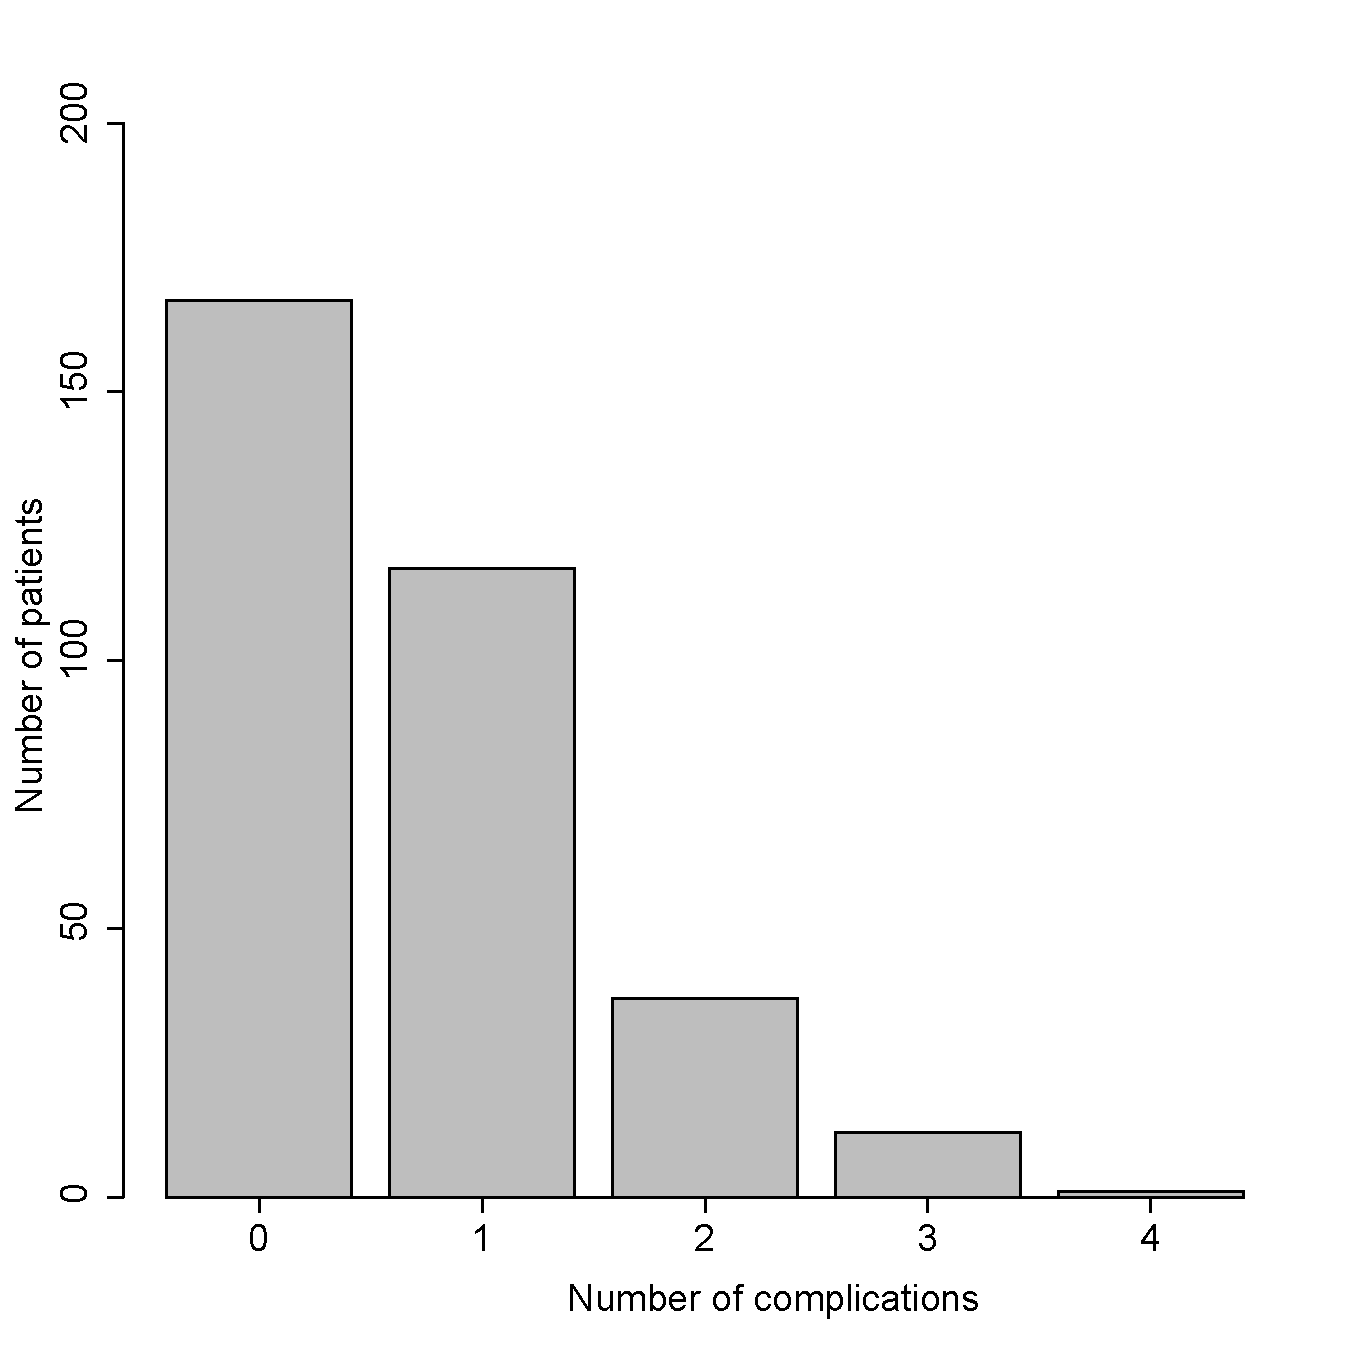
\includegraphics[width=\textwidth]{./Introduction/Barplot_complications_cvid.pdf}%
	\caption{Number of complications}%
\end{subfigure}
\begin{subfigure}[b]{0.49\textwidth}
	\centering
	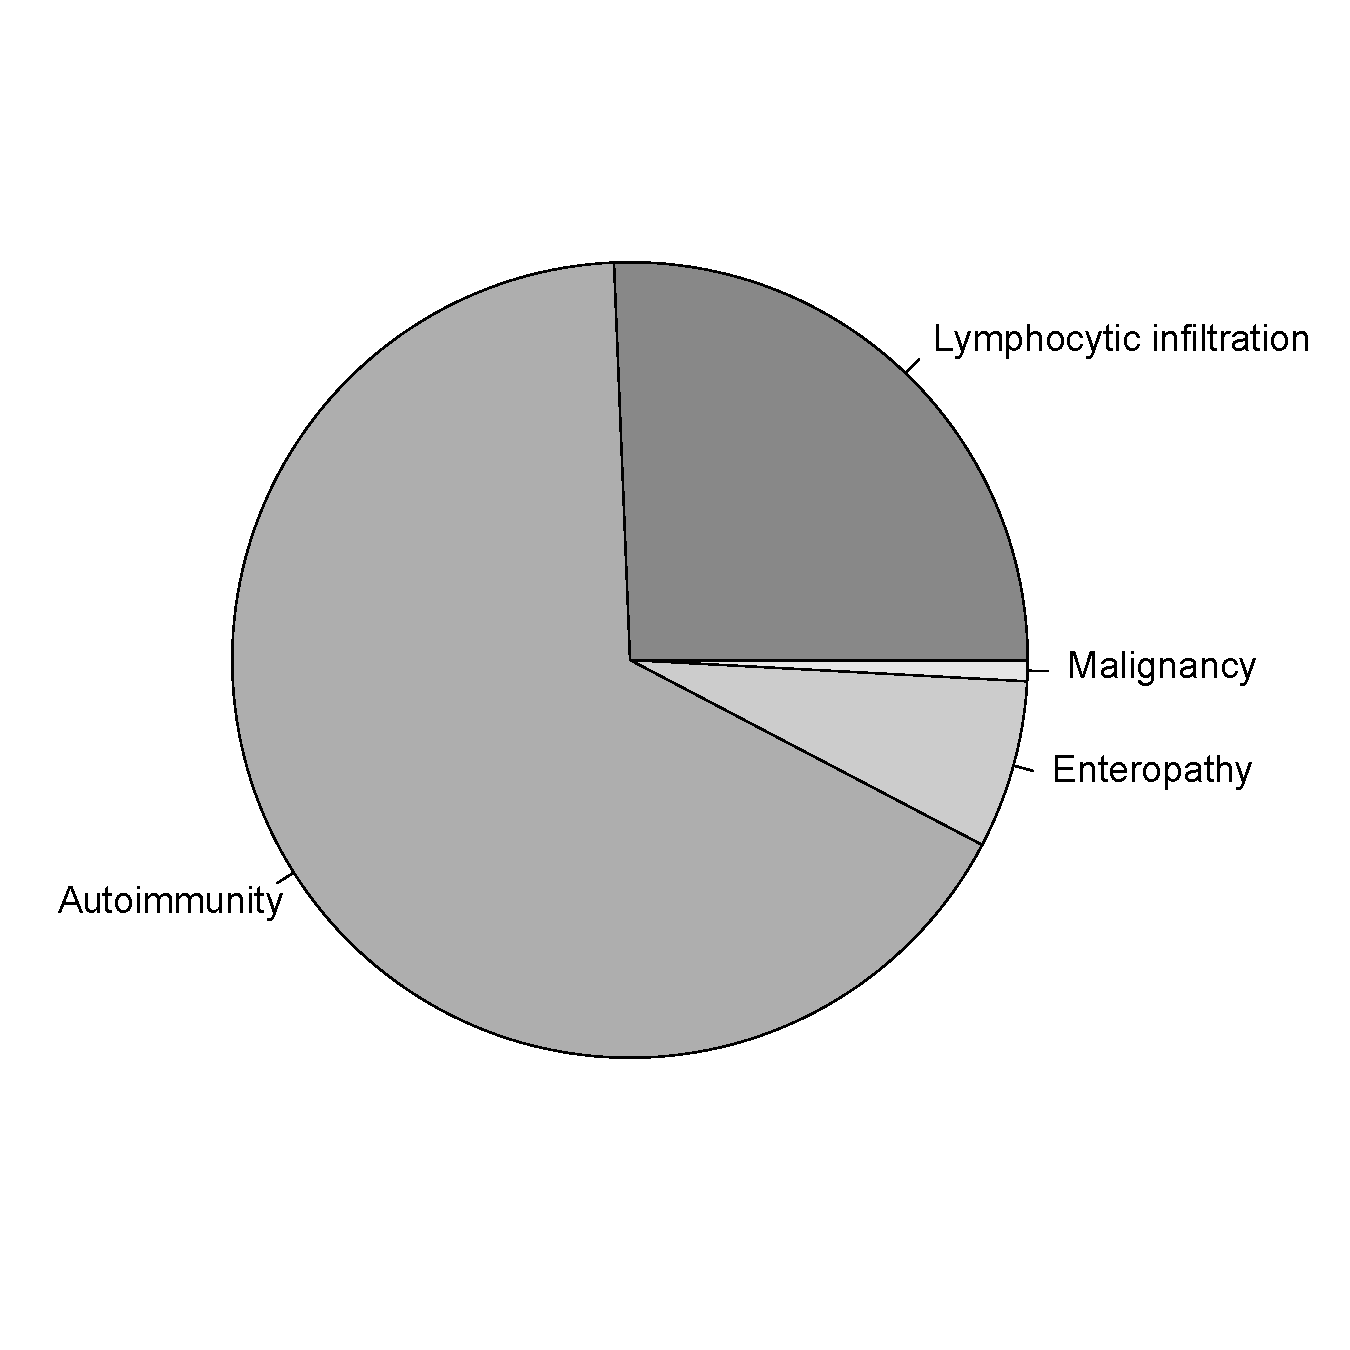
\includegraphics[width=\textwidth]{./Introduction/Pie_1complication.pdf}%
	\caption{One complication}%
\end{subfigure}
\begin{subfigure}[b]{0.49\textwidth}
	\centering
	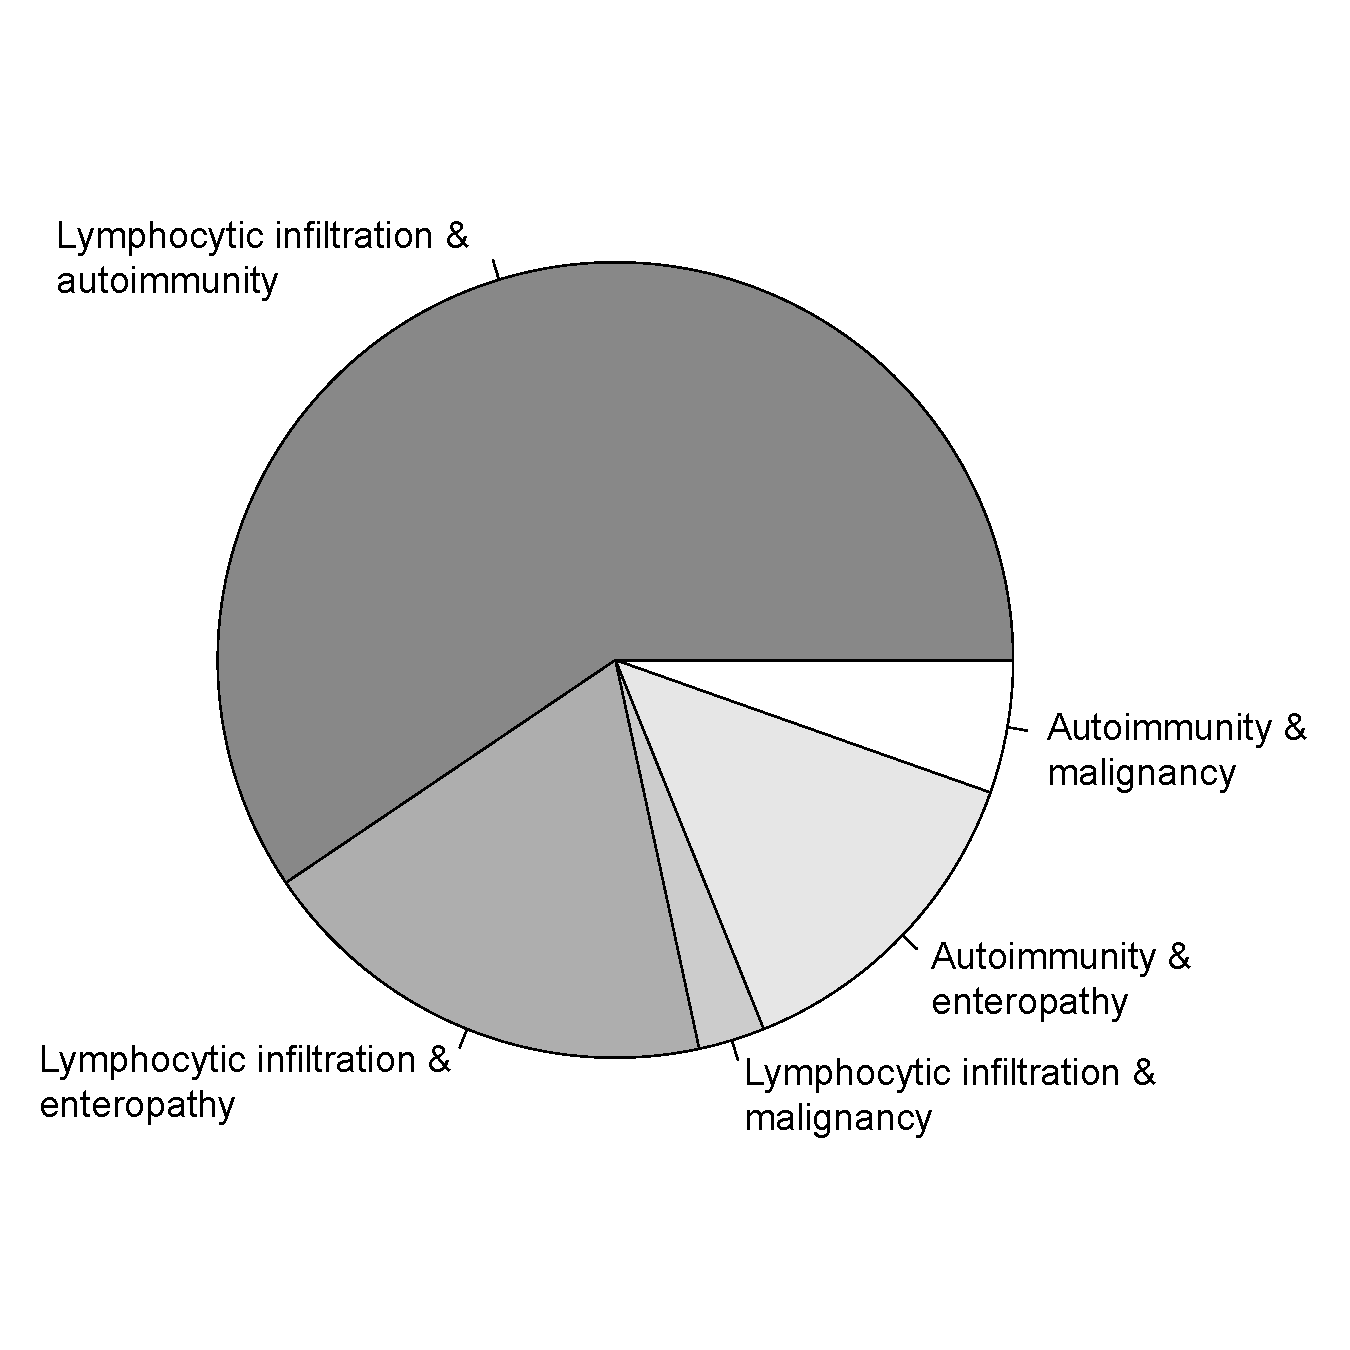
\includegraphics[width=\textwidth]{./Introduction/Pie_2complication.pdf}%
	\caption{Two complications}%
\end{subfigure}
\begin{subfigure}[b]{0.49\textwidth}
	\centering
	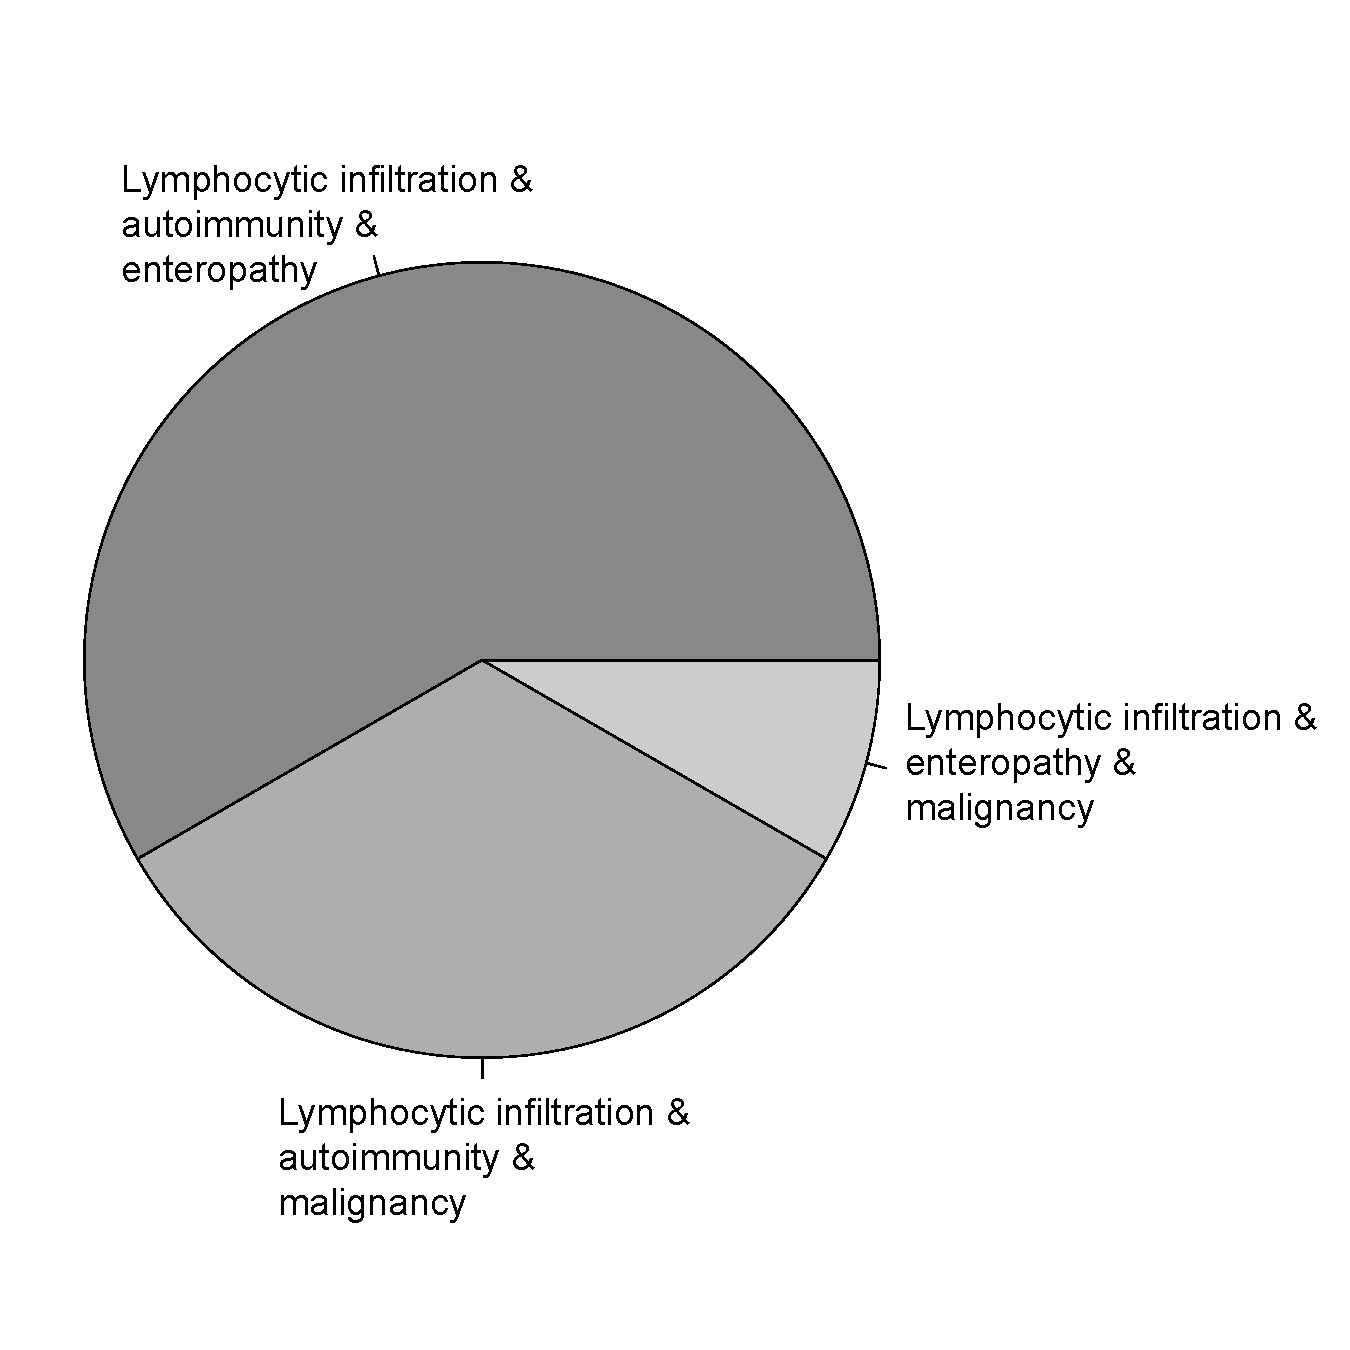
\includegraphics[width=\textwidth]{./Introduction/Pie_3complication.pdf}%
	\caption{Three complications}%
\end{subfigure}
\caption[Nature and number of CVID complications]{\textbf{Nature and number of CVID complications.} a) Number of complications observed in each individual. Individuals with no complications are referred to as infections only. b) Distribution of complications in patients with one complication. c)  Distribution of complications in patients with two complications. d)  Distribution of complications in patients with three complications. \parencite{Chapel2008}}
\label{fig:complications.intro.cvid}
\end{figure}


											% ch:Intro
\appendix
\addcontentsline{toc}{chapter}{Appendices}
\startcontents
\startlist[appendix]{lof}
\startlist[appendix]{lot}
\printcontents{atoc}{0}{\chapter*{Appendices}}
\begingroup
\let\clearpage\relax
\singlespacing
\printlist[appendix]{lof}{}{\chapter*{List of Figures}}
\printlist[appendix]{lot}{}{\chapter*{List of Tables}}
\endgroup

\chapter{Functional genomic response in severe sepsis}
\label{app:expression}

% Table generated by Excel2LaTeX from sheet 'Sheet1'
\clearpage
\begin{table}[H]
  \centering
	\singlespacing
  \caption[Clinical covariates measured for severe sepsis cohort]{\textbf{Clinical covariates measured for severe sepsis cohort.}}
    \begin{tabular}{ll}
    \toprule
   \textbf{ Continuous clinical covariates} & \textbf{Count clinical covariates} \\
    \midrule
    Age   & Sex \\
    Polynucleocytes (raw) & Activated protein C \\
    Mononucleocytes (raw) & Corticosteroid \\
    Lymphocytes (raw) & Microbiology summary \\
    Polynucleocytes (proportion) & Viral infection \\
    Mononucleocytes (proportion) & H1N1 infection \\
    Lymphocytes (proportion) & Ventilation \\
    White cell count & Renal failure \\
    APACHE II & Renal replacement therapy \\
    SOFA (sampling day) & Inotropes \\
    SOFA (maximum recorded) & 14 day survival \\
    Bicarbonate & 28 day survival \\
    Bilirubin & 6 month survival \\
    FIO\textsubscript{2}  &   RNA sampling day \\
    PCO\textsubscript{2}  &  \\
    PAO\textsubscript{2}  &  \\
    Haematocrit &  \\
    Temperature (low) &  \\
    Temperature (high) &  \\
    Heart rate (low) &  \\
    Heart rate (high) &  \\
    Mean arterial pressure (low) &  \\
    Mean arterial pressure (high) &  \\
    Systolic blood pressure (low) &  \\
    Systolic blood pressure (high) &  \\
    Sodium (low) &  \\
    Sodium (high) &  \\
    Potassium (low) & \\
		Potassium (high) & \\
		pH    &  \\
    Platelets &  \\
    Respiratory rate &  \\
    Inotropic support (number of days) &  \\
    Renal support (number of days) &  \\
    Creatinine (high) &  \\
    Creatinine (low) &  \\
		Days in ICU & \\
		Days to death & \\
    \bottomrule
    \end{tabular}%
  \label{tab:app.cov.sepsis}%
\end{table}%



\chapter{Functional genomic response in CVID}
\label{app:CVID}

\clearpage
\begin{center}
\begin{spacing}{1.0}
\begin{longtable}{@{}p{3cm}p{3cm}p{3cm}p{3cm}@{}}
  \caption[Previously described genes for PIDs]{\textbf{Previously described genes for primary immunodeficiency diseases.} \parencite{Bousfiha2013, Al-Herz2011, Milner2013, Stepensky2013, Keller2013}.}
  \label{tab:pid.genes.cvid} \\
		\hline
    \multicolumn{4}{c} {\textbf{Genes}} \\
    \hline
		\endfirsthead
		\multicolumn{4}{c} {\tablename\ \thetable\ -- \textit{Continued from previous page}} \\
		\hline
		\multicolumn{4}{c} {\textbf{Genes}} \\
		\hline
		\endhead
		\hline \multicolumn{4}{c}{\textit{Continued on next page}} \\
		\endfoot 
		\hline
		\endlastfoot
    \textit{ACTB} & \textit{CFI} & \textit{IL2RG} & \textit{PTPRC} \\
    \textit{ADA} & \textit{CIITA} & \textit{IL36RN} & \textit{RAB27a} \\
    \textit{ADAM17} & \textit{COLEC11} & \textit{IL7R} & \textit{RAC2} \\
    \textit{AICDA} & \textit{CORO1A} & \textit{IRAK4} & \textit{RAG1} \\
    \textit{AIRE} & \textit{CSF2RA} & \textit{IRF8} & \textit{RAG2} \\
    \textit{AK2} & \textit{CTSC} & \textit{ISG15} & \textit{RFX 5} \\
    \textit{AP3B} & \textit{CXCR4} & \textit{ITCH} & \textit{RFXANK} \\
    \textit{APOL1} & \textit{CYBA} & \textit{ITGB2} & \textit{RFXAP} \\
    \textit{ATM} & \textit{CYBB} & \textit{ITK} & \textit{RHOH} \\
    \textit{BLM} & \textit{DCLRE1C} & \textit{JAK3} & \textit{RMRP} \\
    \textit{BLNK} & \textit{DKC1} & \textit{KRAS} & \textit{RNF168} \\
    \textit{BTK} & \textit{DNMT3B} & \textit{LCK} & \textit{ROBLD3} \\
    \textit{CEBPE} & \textit{DOCK8} & \textit{LIG4} & \textit{SBDS} \\
    \textit{C15} & \textit{ELANE} & \textit{LPIN2} & \textit{SERPING1} \\
    \textit{C16orf57} & \textit{EVER1} & \textit{LRBA} & \textit{SH2D1A} \\
    \textit{C1QA} & \textit{EVER2} & \textit{LYST} & \textit{SLC35C1} \\
    \textit{C1QB} & \textit{FADD} & \textit{MAGT1} & \textit{SMARCAL1} \\
    \textit{C1QC} & \textit{FAS} & \textit{MASP1} & \textit{SP110} \\
    \textit{C1R} & \textit{FASLG} & \textit{MASP2} & \textit{SPINK5} \\
    \textit{C1S} & \textit{FCN3} & \textit{MBL2} & \textit{STAT1} \\
    \textit{C2} & \textit{FERMT3} & \textit{MCM4} & \textit{STAT3} \\
    \textit{C3} & \textit{FOXN1} & \textit{MEFV} & \textit{STAT5B} \\
    \textit{C4} & \textit{FOXP3} & \textit{MIRL} & \textit{STIM-1} \\
    \textit{C5} & \textit{FPR1} & \textit{MLL2} & \textit{STK4} \\
    \textit{C6} & \textit{G6PC3} & \textit{MRE11} & \textit{STX11} \\
    \textit{C7} & \textit{G6PD} & \textit{MSH5} & \textit{STXBP2} \\
    \textit{C8A} & \textit{G6PT1} & \textit{MTHFD1} & \textit{TAP1} \\
    \textit{C8B} & \textit{GATA2} & \textit{MVK} & \textit{TAP2} \\
    \textit{C9} & \textit{GFI1} & \textit{MYD88} & \textit{TAPBP} \\
    \textit{CARD11} & \textit{HAX1} & \textit{NBS1} & \textit{TAZ} \\
    \textit{CARD9} & \textit{HOIL 1} & \textit{NCF1} & \textit{TBK1} \\
    \textit{CASP10} & \textit{ICOS} & \textit{NCF2} & \textit{TERC} \\
    \textit{CASP8} & \textit{IFNGR1} & \textit{NCF4} & \textit{TERT} \\
    \textit{CD19} & \textit{IFNGR2} & \textit{NHEJ1} & \textit{TINF2} \\
    \textit{CD20} & \textit{IGHM} & \textit{NHP2} & \textit{TLR3} \\
    \textit{CD21} & \textit{IGKC} & \textit{NKX2-5} & \textit{TNFRSF1A} \\
    \textit{CD247} & \textit{IGLL1} & \textit{NLRP3} & \textit{TRAC} \\
    \textit{CD27} & \textit{IKBA} & \textit{NOD2} & \textit{TRAF3} \\
    \textit{CD35} & \textit{IKBkappa} & \textit{NOP10} & \textit{TRIF} \\
    \textit{CD3D} & \textit{IKBKG} & \textit{NRAS} & \textit{TYK2} \\
    \textit{CD3E} & \textit{IKZF1} & \textit{ORAI1} & \textit{UNC119} \\
    \textit{CD3G} & \textit{IL10} & \textit{PFC} & \textit{UNC13D} \\
    \textit{CD40} & \textit{IL10RA} & \textit{PIGA} & \textit{UNC93B1} \\
    \textit{CD40L} & \textit{IL10RB} & \textit{PIK3R1} & \textit{UNG} \\
    \textit{CD46} & \textit{IL12B} & \textit{PLC2G} & \textit{VPS13B} \\
    \textit{CD79A} & \textit{IL12RB1} & \textit{PLDN} & \textit{WAS} \\
    \textit{CD79B} & \textit{IL17F} & \textit{PMS2} & \textit{WIPF1} \\
    \textit{CD81} & \textit{IL17RA} & \textit{PNP} & \textit{XIAP} \\
    \textit{CD8A} & \textit{IL1RN} & \textit{PRF1} & \textit{ZAP70} \\
    \textit{CFD} & \textit{IL21R} & \textit{PRKDC} & \textit{ZBTB24} \\
    \textit{CFH} & \textit{IL2RA} & \textit{PSTPIP1} & \textit{} \\
    \end{longtable}%
		\end{spacing}
		\end{center}
															%

%\bibliographystyle{abbrvnat2}
%\bibliography{Thesis_bibliography2}

\singlespacing
\setlength\bibitemsep{\itemsep}
\printbibliography
\addcontentsline{toc}{chapter}{Bibliography}

\end{document}

% To count text from latex files http://app.uio.no/ifi/texcount/online.php
% Up to 300 pages for soft binding